\documentclass[tikz,border=3pt]{standalone}
\usepackage{amsmath,amssymb}
\usetikzlibrary{arrows.meta,positioning,calc,fit,backgrounds}

\definecolor{ink}{HTML}{243447}
\definecolor{blue}{HTML}{4477AA}
\definecolor{cyan}{HTML}{66CCEE}
\definecolor{green}{HTML}{228833}
\definecolor{gold}{HTML}{CCBB44}
\definecolor{rose}{HTML}{CC6677}
\definecolor{lightblue}{HTML}{EAF2F8}
\definecolor{lightgold}{HTML}{FAF6DF}
\definecolor{papergray}{HTML}{F5F6F7}

\begin{document}
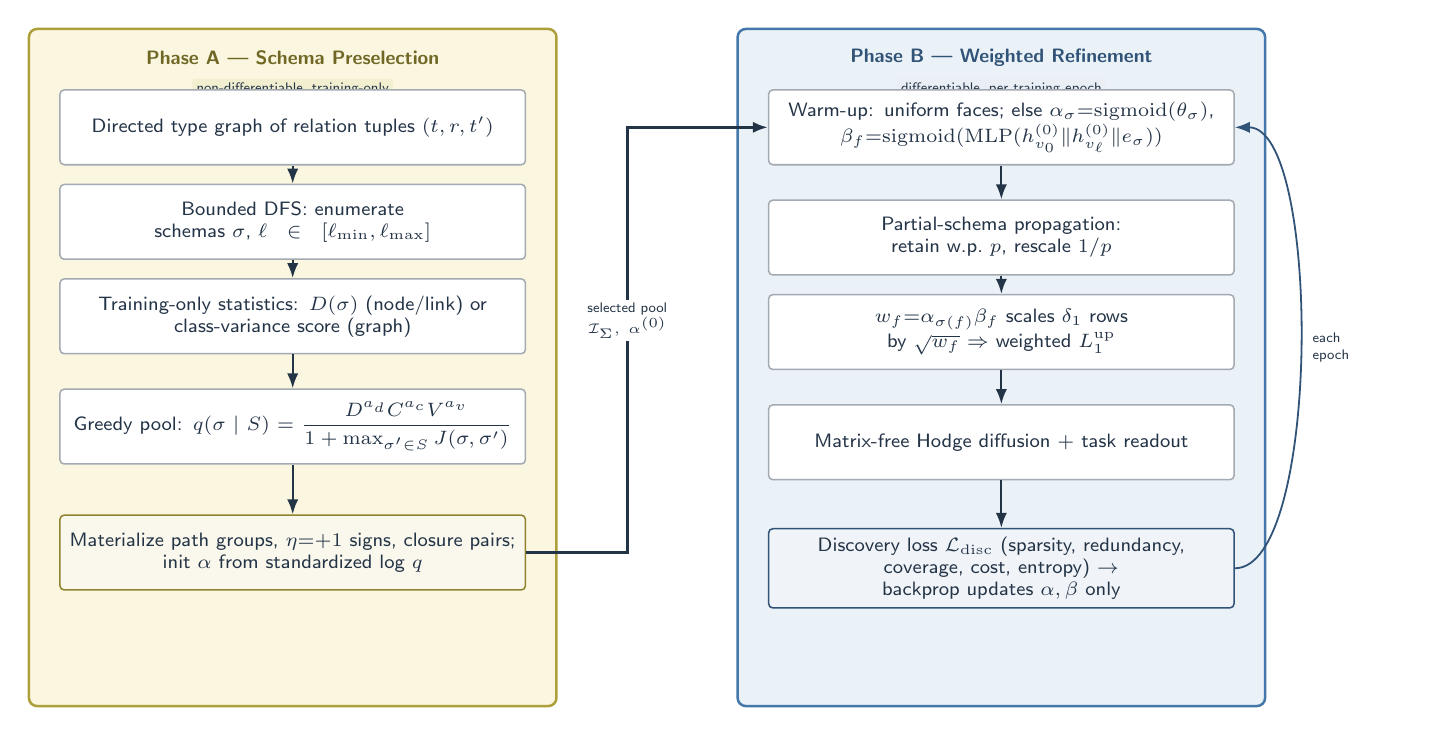
\begin{tikzpicture}[
  font=\sffamily\scriptsize,
  text=ink,
  >=Latex,
  flow/.style={-{Latex[length=1.9mm]},draw=ink,line width=0.8pt},
  stage/.style={rounded corners=3pt,line width=0.9pt,minimum width=6.7cm,
    minimum height=8.6cm,inner sep=5pt,align=center},
  item/.style={rounded corners=1.5pt,draw=ink!42,fill=white,line width=0.55pt,
    text width=5.7cm,minimum height=0.95cm,align=center,inner sep=3pt}
]

% =====================================================================
% Phase A — preprocessing (non-differentiable, training-only)
% =====================================================================
\node[stage,draw=gold!85!black,fill=lightgold] (phaseA) at (0,0) {};
\node[font=\sffamily\bfseries\scriptsize,gold!55!black] at ($(phaseA.north)+(0,-0.38)$)
  {Phase A --- Schema Preselection};
\node[font=\sffamily\tiny,fill=gold!25,rounded corners=1pt,inner sep=1.5pt]
  at ($(phaseA.north)+(0,-0.78)$) {non-differentiable, training-only};

\node[item] (a1) at ($(phaseA.center)+(0,3.05)$)
  {Directed type graph of relation tuples $(t,r,t')$};
\node[item] (a2) at ($(phaseA.center)+(0,1.85)$)
  {Bounded DFS: enumerate schemas $\sigma$,\ $\ell\in[\ell_{\min},\ell_{\max}]$};
\node[item] (a3) at ($(phaseA.center)+(0,0.65)$)
  {Training-only statistics: $D(\sigma)$ (node/link) or\\ class-variance score (graph)};
\node[item] (a4) at ($(phaseA.center)+(0,-0.75)$)
  {Greedy pool: $q(\sigma\mid S)=\dfrac{D^{a_d}C^{a_c}V^{a_v}}{1+\max_{\sigma'\in S}J(\sigma,\sigma')}$};
\node[item,draw=gold!70!black,fill=gold!10] (a5) at ($(phaseA.center)+(0,-2.35)$)
  {Materialize path groups, $\eta{=}{+}1$ signs, closure pairs;\\ init $\alpha$ from standardized log $q$};

\draw[flow] (a1) -- (a2);
\draw[flow] (a2) -- (a3);
\draw[flow] (a3) -- (a4);
\draw[flow] (a4) -- (a5);

% =====================================================================
% Phase B — training loop (differentiable after the pool is fixed)
% =====================================================================
\node[stage,draw=blue,fill=lightblue] (phaseB) at (9.0,0) {};
\node[font=\sffamily\bfseries\scriptsize,blue!70!black] at ($(phaseB.north)+(0,-0.38)$)
  {Phase B --- Weighted Refinement};
\node[font=\sffamily\tiny,fill=blue!12,rounded corners=1pt,inner sep=1.5pt]
  at ($(phaseB.north)+(0,-0.78)$) {differentiable, per training epoch};

\node[item] (b1) at ($(phaseB.center)+(0,3.05)$)
  {Warm-up: uniform faces; else $\alpha_\sigma{=}\mathrm{sigmoid}(\theta_\sigma)$,\\
   $\beta_f{=}\mathrm{sigmoid}(\mathrm{MLP}(h_{v_0}^{(0)}\Vert h_{v_\ell}^{(0)}\Vert e_\sigma))$};
\node[item] (b2) at ($(phaseB.center)+(0,1.65)$)
  {Partial-schema propagation: retain w.p.\ $p$, rescale $1/p$};
\node[item] (b3) at ($(phaseB.center)+(0,0.45)$)
  {$w_f{=}\alpha_{\sigma(f)}\beta_f$ scales $\delta_1$ rows by $\sqrt{w_f}$
   $\Rightarrow$ weighted $L_1^{\mathrm{up}}$};
\node[item] (b4) at ($(phaseB.center)+(0,-0.95)$)
  {Matrix-free Hodge diffusion $+$ task readout};
\node[item,draw=blue!70!black,fill=blue!8] (b5) at ($(phaseB.center)+(0,-2.55)$)
  {Discovery loss $\mathcal L_{\mathrm{disc}}$ (sparsity, redundancy,\\
   coverage, cost, entropy) $\to$ backprop updates $\alpha,\beta$ only};

\draw[flow] (b1) -- (b2);
\draw[flow] (b2) -- (b3);
\draw[flow] (b3) -- (b4);
\draw[flow] (b4) -- (b5);
\draw[flow,draw=blue!70!black,line width=0.65pt]
  (b5.east) .. controls +(1.1,0) and +(1.1,0) .. (b1.east)
  node[midway,right=1pt,font=\sffamily\tiny,align=left,text width=1.3cm] {each\\ epoch};

% =====================================================================
% Bridge: selected pool feeds the training loop
% =====================================================================
\draw[flow,line width=1.0pt] (a5.east) -- (4.25,-2.35) -- (4.25,3.05) -- (b1.west);
\node[font=\sffamily\tiny,align=center,fill=white,inner sep=1pt, text width=1.7cm]
  at (4.25,0.6) {selected pool\\ $\mathcal I_\Sigma,\ \alpha^{(0)}$};

\end{tikzpicture}
\end{document}
